%\begin{document}
\chapter*{Введение}
\markboth{Введение}{ }

\addcontentsline{toc}{chapter}{Введение}
Полярные мезоциклоны продолжают привлекать к себе внимание исследователей благодаря своей сложной динамике, отличающейся от циклонов тропических широт. Эти мезомасштабные вихри являются короткоживущими объектами, которые образуются в арктических и антарктических морях, где данные метеорологических наблюдений достаточно разрежены. Поэтому эволюция полярных мезоциклонов представляется сложной задачей для численного прогноза ввиду недостатка начальных и граничных условий, а также из-за большой чувствительности к малым возмущениям в пограничном слое атмосферы.

Зарождение полярных мезоциклонов все еще остается предметом научных дискуссий. Причиной этому видится большое разнообразие мезоциклонов по структуре и жизненному циклу, возникающих в самых разных частях Мирового океана: от моря Лабрадор до Японского и от Норвежского до моря Уэделла. Большой разброс параметров окружающей атмосферы существенно усложняет как теоретическое, так и численное моделирование этих вихрей. Поэтому за последние десятилетия накопилось множество статей, авторы которых рассматривают влияние на эволюцию мезоциклонов таких факторов, как степень бароклинности (т. е. горизонтальная термическая неоднородность), устойчивость атмосферы (т. е. вертикальный градиент температуры), параметры подстилающей поверхности, включая распределение льда, температура поверхности воды, потоки явного и скрытого тепла, наличие барической аномалии в верхней тропосфере. Исходя из этого, были предложены различные механизмы зарождения полярных вихрей. Тот или иной механизм обычно в одиночку не мог объяснить развитие выбранного мезоциклона, и был сделан вывод, что несколько процессов действуют одновременно в течение времени жизни мезоциклона.

\section*{Подходы к моделированию механизмов развития мезоциклонов}
\addcontentsline{toc}{section}{Подходы к моделированию механизмов развития мезоциклонов}
Не затрагивая работы, посвященные описанию конкретных наблюдаемых мезоциклонов, остановимся на тех, которые основаны на моделировании. Используемые в них подходы условно можно разделить на три группы. Обозначим основные достоинства и недостатки того или иного метода.
\begin{sqlist}
\item Теоретическое (аналитическое) моделирование \\
Преимуществом является отсутствие требований к вычислительным ресурсам и отсутствие вычислительных ошибок, а главное, возможность уверенно разделить влияние того или иного источника развития мезоциклона путем исключения его из уравнений. Однако аналитические модели чаще всего строятся на упрощенных линеаризованных уравнениях, в которых особенно плохо представлена конвекция. 

\item Численное моделирование по данным наблюдений ('case studies') \\
Данный тип исследований преобладает по количеству. В большинстве таких работ фокус сделан на конкретный наблюдаемый вихрь, формирование которого подвержено одновременно многим факторам, влияние которых сложно отделить друг от друга. Тем не менее, подход 'case study' позволяет максимально приблизить результаты моделирования к данным наблюдений и провести валидацию модели, настроив ее для численного прогноза погоды в выбранном регионе.

\item Идеализированные численные эксперименты \\
В качестве подхода к теории динамики мезоциклонов идеализированное моделирование в достаточной степени объединяет в себе достоинства первых двух методов и позволяет глубоко вникнуть в суть нелинейных процессов. Именно этот подход используется в данной курсовой работе.
Здесь необходимо отметить, что широко используемый способ проведения численных экспериментов, подразумевающий отключение какого-либо физического процесса, имеет следующие недостатки \citep{YanaseEtAl2004}: при длительном отсутствии какого-либо процесса меняется не только динамика вихря, но и состояние окружающей его атмосферы, что косвенным образом отражается на исследуемом объекте.
\end{sqlist}

\section*{Объект и цель исследования}
\addcontentsline{toc}{section}{Объект и цель исследования}
Объектом работы являются полярные мезоциклоны, развитие которых определяет термическая неустойчивость. Уже в первых теоретических исследованиях было замечено, что конвекция играет важную роль в развитии полярных вихрей. Уже в пионерных работах (например, \citep{BusingerReed1989}) отмечалось, что облачные системы полярных мезоциклонов в значительной степени имеют конвективную природу. В пользу этой точки зрения говорят и многочисленные спутниковые снимки. 

\begin{figure}
  \centering
  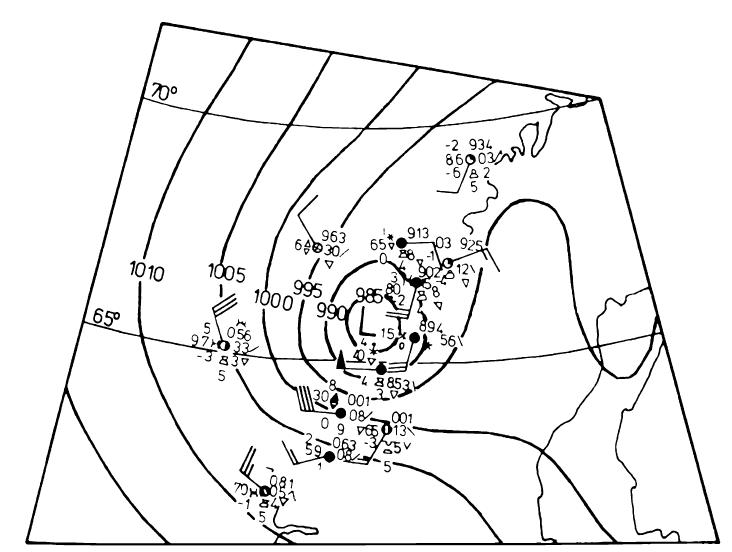
\includegraphics[width=0.5\linewidth]{{./chapters/figures_misc/polarlow1971}.jpeg}
  \caption{Синоптическая карта приземного анализа, показывающая наличие полярного мезоциклона в Норвежском море вблизи побережья Норвегии 13 октября 1971 г. \citep{RT2003}.}
  \label{fig:polarlow1971}
\end{figure}

Ярким примером является полярный мезомасштабный циклон, наблюдавшийся вблизи побережья Норвегии вблизи полярного круга 13 октября 1971 года \citep{Rasmussen1979}. На ранних стадиях его развития отмечалось большое количество энергии неустойчивости и формирование обширных систем глубокой конвекции, что привело к образованию осесимметричного вихря с теплым ядром, замкнутой циркуляцией диаметром несколько сотен километров и со скоростями приземного ветра, в среднем равными $25\mps$ (рис. \ref{fig:polarlow1971}).

Целью данной работы является исследование механизмов формирования полярных мезоциклонов на начальных стадиях их эволюции. Акцент сделан на воздействие параметров атмосферы, потому что динамика мезоциклонов любого типа зависит от благоприятных условий окружающей атмосферы. Будет показано, какое начальное состояние атмосферы благоприятно для генерации вихря в терминах изменения его кинетической энергии и падения приземного давления.

Для достижения поставленной в работе цели решаются следующие задачи:
\begin{sqlist}
\item Изучение зависимости характеристик полярного мезоциклона от внешних метеорологических параметров в их широком диапазоне. Одним из результатов решения задачи является определение области метеовеличин, благоприятной для интенсификации циклонического возмущения.
\item Выявление эффекта использования в модели той или иной параметризации турбулентного перемешивания в приводном и пограничном слоях атмосферы на динамику и структуру циркуляции.
\end{sqlist}

\subsubsection*{Структура дипломной работы}
Дипломная работа состоит из введения, трех глав, заключения, библиографии и приложения. В первой главе на основе обзора литературы рассматриваются основные физические механизмы, объясняющие зарождение и эволюцию полярных мезоциклонов. Во второй главе описывается численная мезомасштабная модель ReMeDy, а именно система уравнений и используемые параметризации. Далее производится постановка стратегии исследования и выбор метода исследования. В частности, особое внимание уделяется энергетической диагностике. В четвертой главе приводятся результаты серий численных экспериментов, анализируются возникающие мезомасштабные циркуляции и объясняется их динамика. Кроме того, приводятся количественные оценки чувствительности интенсивности полярного мезоциклона к внешним параметрам атмосферы и к используемым параметризациям. В заключении содержатся основные выводы работы и обсуждается их теоретическая значимость. Приложение включает вывод системы уравнений мезомасштабной модели ReMeDy.

%\end{document}